\documentclass[11pt,a4paper]{article}
\usepackage[utf8]{inputenc}
\usepackage{amsmath,amsfonts,amssymb}
\usepackage{graphicx}
\usepackage{geometry}
\geometry{margin=1in}
\usepackage{booktabs}
\usepackage{hyperref}
\usepackage{float}
\usepackage{xcolor}

\definecolor{darkbg}{HTML}{0d121f}
\definecolor{lighttext}{HTML}{e2e8f0}
\definecolor{primary}{HTML}{8b5cf6}
\definecolor{secondary}{HTML}{0dd5c5}

\pagecolor{darkbg}
\color{lighttext}

\hypersetup{
    colorlinks=true,
    linkcolor=secondary,
    urlcolor=secondary
}

\title{\textbf{EE3621: Digital Signal Processing} \\ \Large Lecture 8: Properties of the DFT \& Circular Convolution \\ \large (III B.Tech EEE)}
\author{Lecture Notes (40-Minute Plan)}
\date{}

\begin{document}

\maketitle

\section{Lecture Plan \& Objectives (40 Minutes Breakdown)}
\begin{itemize}
    \item \textbf{00:00 -- 05:00 (5 mins):} Motivation: Why study DFT properties? (FFT derivations and filtering applications).
    \item \textbf{05:00 -- 15:00 (10 mins):} Fundamental properties: Periodicity, Linearity, and Conjugate Symmetry.
    \item \textbf{15:00 -- 25:00 (10 mins):} Circular Shift of a sequence in time and frequency domains; comparison with linear shift.
    \item \textbf{25:00 -- 35:00 (10 mins):} Circular Convolution -- definition, properties, and comparison with linear convolution. Matrix methods.
    \item \textbf{35:00 -- 40:00 (5 mins):} Parseval's Theorem, Review checkpoints, and Q\&A.
\end{itemize}

\noindent\rule{\textwidth}{0.5pt}

\section{Fundamental Properties of the DFT}

Let $x[n] \longleftrightarrow X[k]$ represent an $N$-point DFT pair, defined as:
\begin{align}
X[k] &= \sum_{n=0}^{N-1} x[n] W_N^{kn} \\
x[n] &= \frac{1}{N} \sum_{k=0}^{N-1} X[k] W_N^{-kn}
\end{align}
where $W_N = e^{-j\frac{2\pi}{N}}$ is the twiddle factor.

\subsection{Periodicity}
\textbf{Theorem (Periodicity):} If $x[n]$ and $X[k]$ form an $N$-point DFT pair, then they are implicitly periodic with period $N$:
\begin{align}
X[k+N] &= X[k] \\
x[n+N] &= x[n]
\end{align}

\textbf{Proof for Frequency Domain ($X[k+N] = X[k]$):}
\begin{align}
X[k+N] &= \sum_{n=0}^{N-1} x[n] W_N^{(k+N)n} \\
&= \sum_{n=0}^{N-1} x[n] W_N^{kn} W_N^{Nn}
\end{align}
Since $W_N = e^{-j\frac{2\pi}{N}}$, we have $W_N^{Nn} = \left(e^{-j\frac{2\pi}{N}}\right)^{Nn} = e^{-j2\pi n} = 1$. Substituting this back:
\begin{equation}
X[k+N] = \sum_{n=0}^{N-1} x[n] W_N^{kn} (1) = X[k]
\end{equation}

\textbf{Proof for Time Domain ($x[n+N] = x[n]$):}
\begin{align}
x[n+N] &= \frac{1}{N} \sum_{k=0}^{N-1} X[k] W_N^{-k(n+N)} \\
&= \frac{1}{N} \sum_{k=0}^{N-1} X[k] W_N^{-kn} W_N^{-kN}
\end{align}
Since $W_N^{-kN} = e^{j2\pi k} = 1$ for any integer $k$:
\begin{equation}
x[n+N] = \frac{1}{N} \sum_{k=0}^{N-1} X[k] W_N^{-kn} = x[n]
\end{equation}

\textbf{Engineering Intuition:} Sampling in the frequency domain inherently causes a periodic extension in the time domain. A finite sequence is treated as one period of a periodic signal.

\subsection{Conjugate Symmetry (Hermitian Symmetry)}
\textbf{Theorem (Symmetry for Real Signals):} If $x[n]$ is real ($x[n] = x^*[n]$), then the DFT exhibits conjugate symmetry: $X[k] = X^*[N-k]$.

\textbf{Proof:}
\begin{equation}
X[k] = \sum_{n=0}^{N-1} x[n] e^{-j \frac{2\pi}{N} kn}
\end{equation}
Taking the complex conjugate:
\begin{equation}
X^*[k] = \sum_{n=0}^{N-1} x^*[n] e^{j \frac{2\pi}{N} kn} = \sum_{n=0}^{N-1} x[n] e^{j \frac{2\pi}{N} kn}
\end{equation}
Now evaluate $X[N-k]$:
\begin{align}
X[N-k] &= \sum_{n=0}^{N-1} x[n] e^{-j \frac{2\pi}{N} (N-k)n} \\
&= \sum_{n=0}^{N-1} x[n] e^{-j 2\pi n} e^{j \frac{2\pi}{N} kn}
\end{align}
Since $e^{-j 2\pi n} = 1$:
\begin{equation}
X[N-k] = \sum_{n=0}^{N-1} x[n] e^{j \frac{2\pi}{N} kn} = X^*[k]
\end{equation}

\textbf{Consequences of Symmetry:}
\begin{itemize}
    \item \textbf{DC Value:} $k=0 \implies X[0] = \sum x[n]$. Purely real.
    \item \textbf{Nyquist Bin:} If $N$ is even, $k=N/2$ is purely real since $X[N/2] = X^*[N/2]$.
    \item \textbf{One-sided Spectrum:} For $N$ samples, bins from $k=1$ to $N/2-1$ contain all unique frequency information.
\end{itemize}

\section{Circular Shift of a Sequence}

\subsection{Definition of Circular Shift}
A circular shift of $x[n]$ by $m$ samples is denoted using modulo indexing:
\begin{equation}
x_c[n] = x[((n - m))_N]
\end{equation}

\begin{figure}[H]
\centering
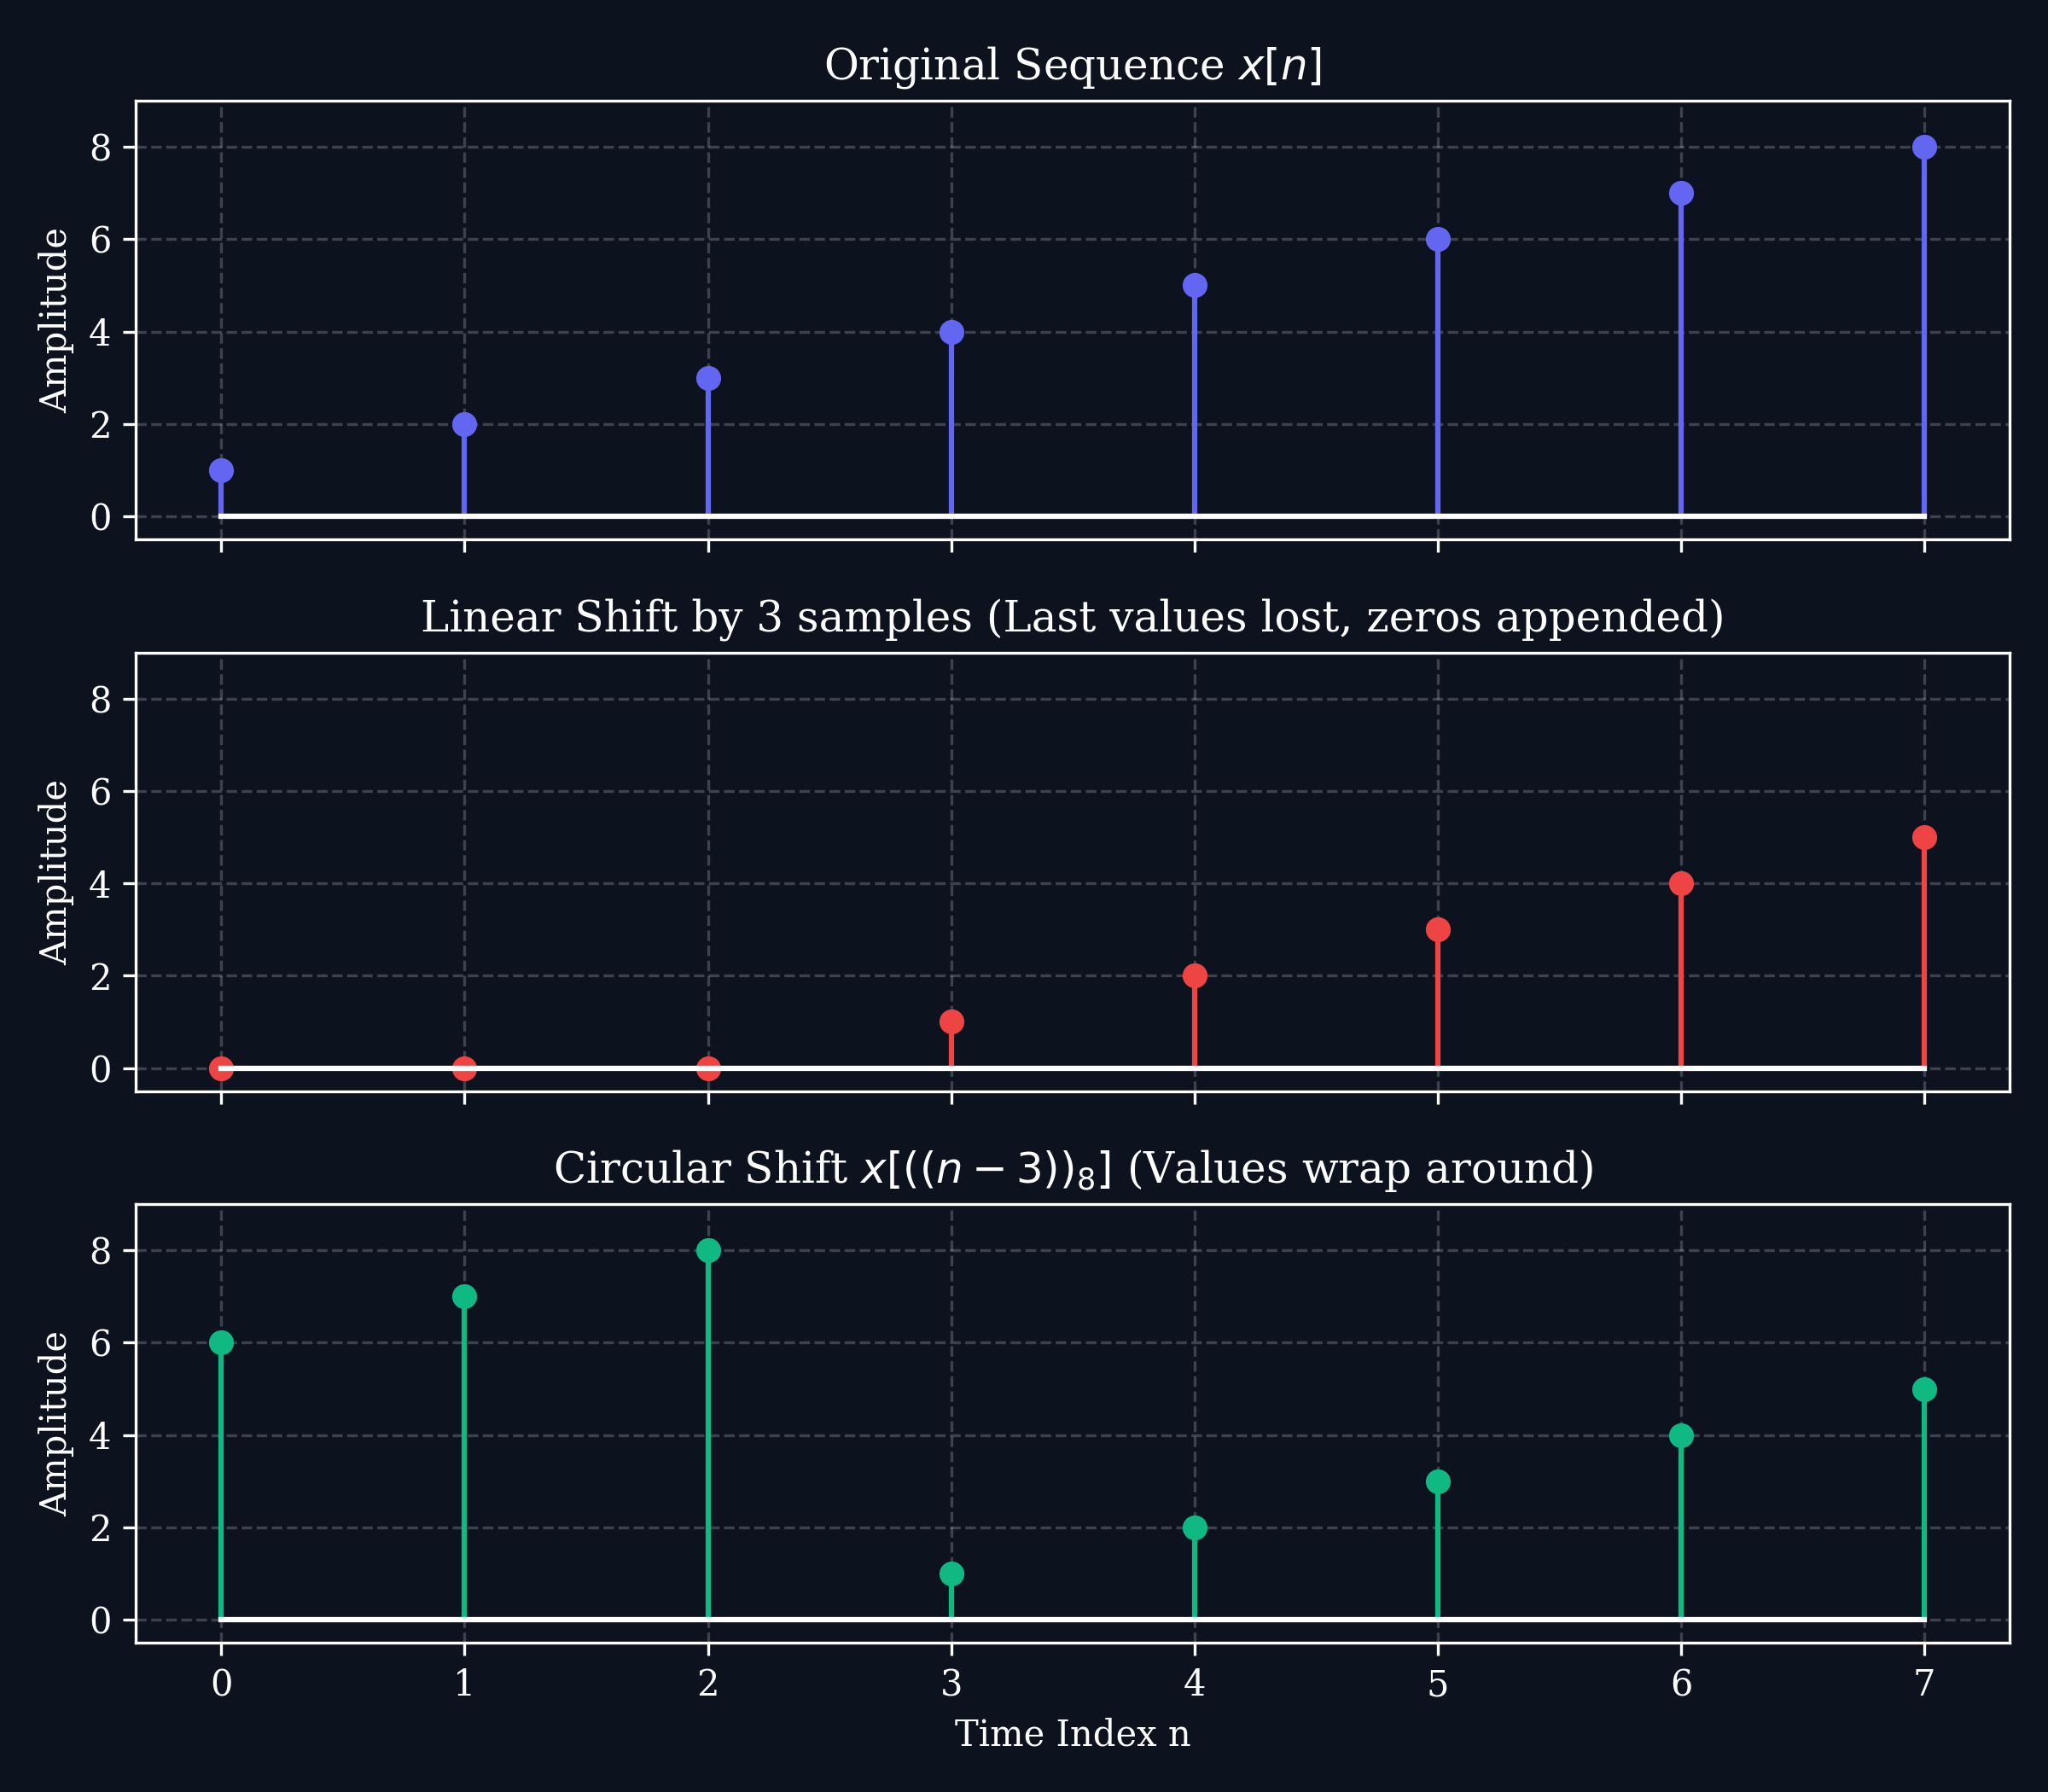
\includegraphics[width=0.85\textwidth]{images/circular_shift_comparison.png}
\caption{Comparison of Linear Shift vs. Circular Shift ($N=8$, shift $m=3$).}
\label{fig:shift_comp}
\end{figure}

\subsection{Circular Time Shift Theorem}
\begin{equation}
x[((n - m))_N] \longleftrightarrow X[k] W_N^{km}
\end{equation}

\textbf{Proof:}
\begin{equation}
X_c[k] = \sum_{n=0}^{N-1} x[((n-m))_N] W_N^{kn}
\end{equation}
Let $l = n - m \implies n = l + m$:
\begin{align}
X_c[k] &= \sum_{l=0}^{N-1} x[((l))_N] W_N^{k(l+m)} \\
&= W_N^{km} \sum_{l=0}^{N-1} x[l] W_N^{kl} \\
&= W_N^{km} X[k]
\end{align}

\section{Circular Convolution}

\subsection{Mathematical Definition}
The circular convolution of $x_1[n]$ and $x_2[n]$ of length $N$ is:
\begin{equation}
y[n] = x_1[n] \circledast_N x_2[n] = \sum_{m=0}^{N-1} x_1[m] x_2[((n - m))_N], \quad 0 \le n \le N-1
\end{equation}

\subsection{Circular Convolution Theorem}
\begin{equation}
y[n] = x_1[n] \circledast_N x_2[n] \longleftrightarrow Y[k] = X_1[k] \cdot X_2[k]
\end{equation}

\textbf{Proof:}
\begin{align}
Y[k] &= \sum_{n=0}^{N-1} \left[ \sum_{m=0}^{N-1} x_1[m] x_2[((n - m))_N] \right] W_N^{kn} \\
&= \sum_{m=0}^{N-1} x_1[m] \left[ \sum_{n=0}^{N-1} x_2[((n - m))_N] W_N^{kn} \right] \\
&= \sum_{m=0}^{N-1} x_1[m] \left[ X_2[k] W_N^{km} \right] \\
&= X_2[k] \sum_{m=0}^{N-1} x_1[m] W_N^{km} \\
&= X_2[k] \cdot X_1[k]
\end{align}

\subsection{Circulant Matrix Representation}
The operation $y = x_1 \circledast_N x_2$ is equivalent to $\mathbf{y} = \mathbf{H} \mathbf{x_1}$, where $\mathbf{H}$ is a circulant matrix:
\begin{equation}
\begin{bmatrix} y[0] \\ y[1] \\ y[2] \\ \vdots \\ y[N-1] \end{bmatrix} = 
\begin{bmatrix} 
x_2[0] & x_2[N-1] & x_2[N-2] & \cdots & x_2[1] \\ 
x_2[1] & x_2[0] & x_2[N-1] & \cdots & x_2[2] \\ 
x_2[2] & x_2[1] & x_2[0] & \cdots & x_2[3] \\ 
\vdots & \vdots & \vdots & \ddots & \vdots \\ 
x_2[N-1] & x_2[N-2] & x_2[N-3] & \cdots & x_2[0] 
\end{bmatrix} 
\begin{bmatrix} x_1[0] \\ x_1[1] \\ x_1[2] \\ \vdots \\ x_1[N-1] \end{bmatrix}
\end{equation}
The eigenvalues of this circulant matrix are exactly the DFT coefficients $X_2[k]$.

\subsection{Linear vs. Circular Convolution (Time Aliasing)}
If linear convolution is $y_{lin}[n] = x_1[n] * x_2[n]$, circular convolution is:
\begin{equation}
y_{circ}[n] = \sum_{r=-\infty}^{\infty} y_{lin}[n - rN], \quad 0 \le n \le N-1
\end{equation}

\textbf{Zero-Padding Rule:} If $N \ge L_1 + L_2 - 1$, $y_{circ}[n] = y_{lin}[n]$. Otherwise, aliasing occurs.

\begin{figure}[H]
\centering
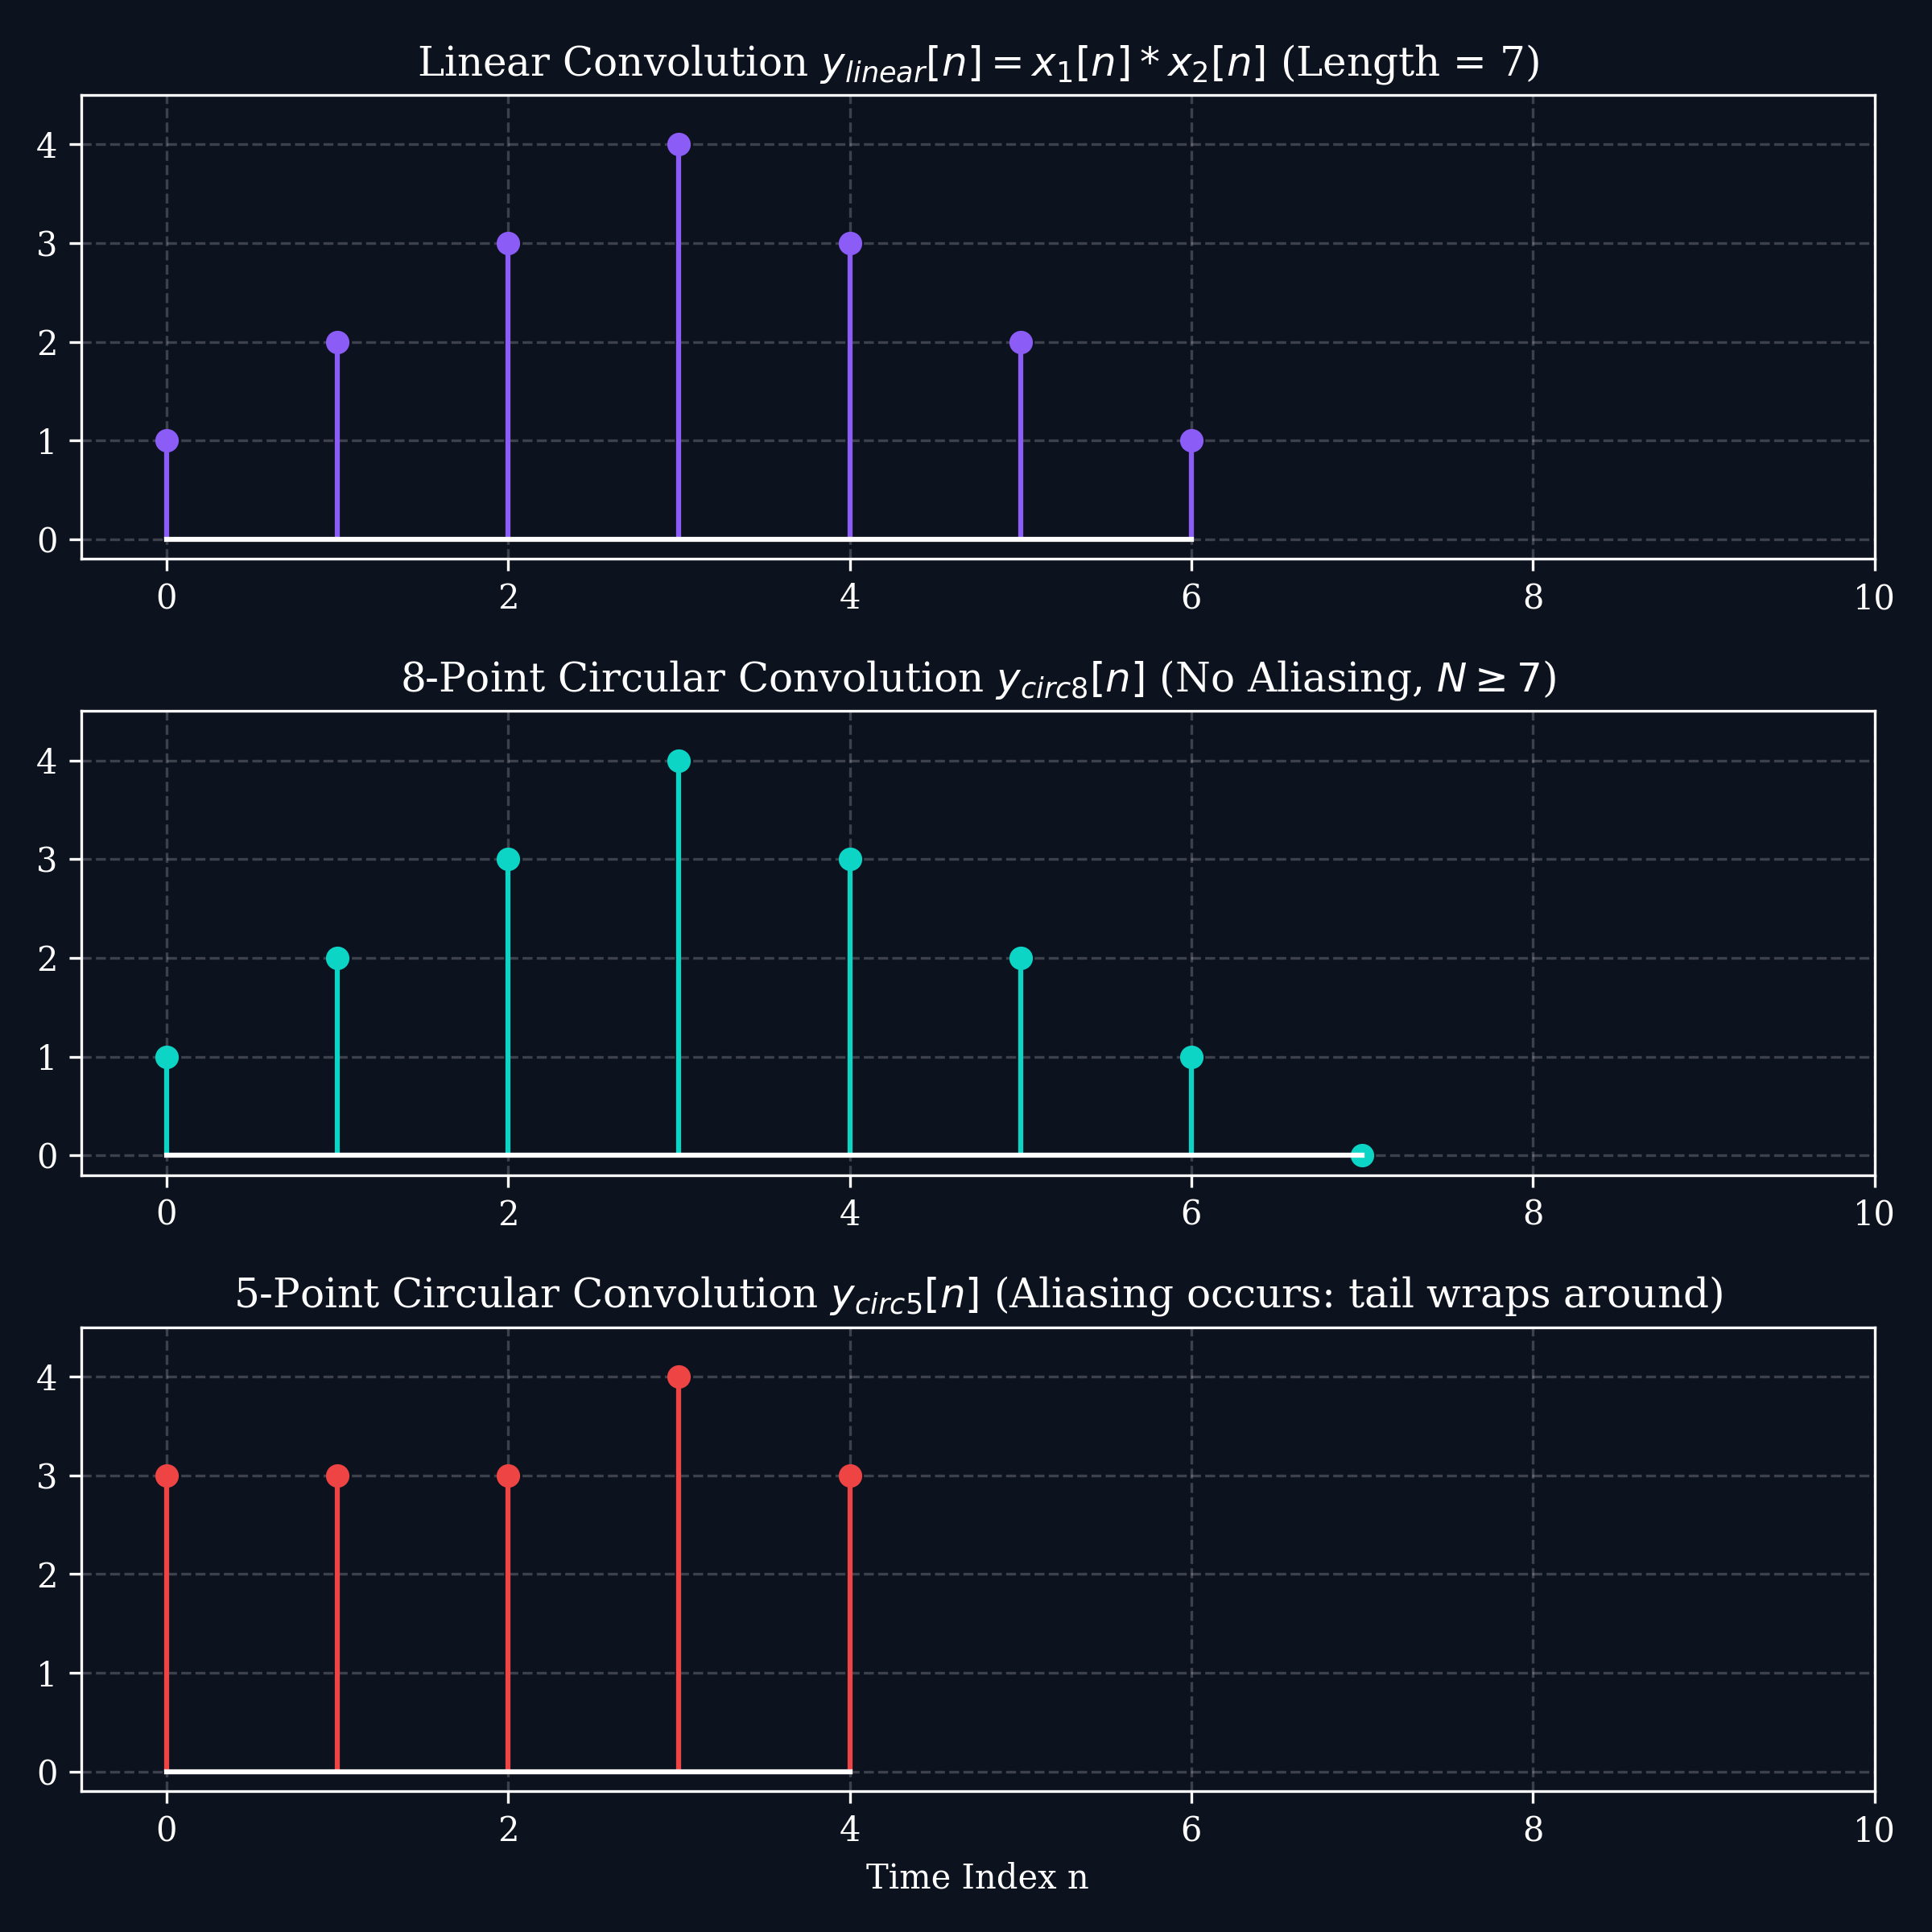
\includegraphics[width=0.85\textwidth]{images/circular_vs_linear_convolution.png}
\caption{Comparison of Linear Convolution and Circular Convolution.}
\label{fig:conv_comp}
\end{figure}

\subsection{Full Numerical Example: 4-Point Circular Convolution}
Let $x_1[n] = \{1, 2, 3, 4\}$ and $x_2[n] = \{1, 0, 1, 0\}$. Find $y[n] = x_1[n] \circledast_4 x_2[n]$.

\textbf{Method 1: Circulant Matrix Approach}
\begin{equation}
\begin{bmatrix} y[0] \\ y[1] \\ y[2] \\ y[3] \end{bmatrix} = \begin{bmatrix} 1 & 0 & 1 & 0 \\ 0 & 1 & 0 & 1 \\ 1 & 0 & 1 & 0 \\ 0 & 1 & 0 & 1 \end{bmatrix} \begin{bmatrix} 1 \\ 2 \\ 3 \\ 4 \end{bmatrix} = \begin{bmatrix} 4 \\ 6 \\ 4 \\ 6 \end{bmatrix}
\end{equation}
So, $y[n] = \{4, 6, 4, 6\}$.

\textbf{Method 2: DFT Multiplication Approach}
\begin{itemize}
    \item $X_1[k] = \{10, -2+j2, -2, -2-j2\}$
    \item $X_2[k] = \{2, 0, 2, 0\}$
    \item $Y[k] = X_1[k]X_2[k] = \{20, 0, -4, 0\}$
    \item $y[n] = \text{IDFT}(Y[k]) = \{4, 6, 4, 6\}$
\end{itemize}

\section{Parseval's Theorem for DFT}

\textbf{Theorem:}
\begin{equation}
\sum_{n=0}^{N-1} |x[n]|^2 = \frac{1}{N} \sum_{k=0}^{N-1} |X[k]|^2
\end{equation}

\textbf{Proof:}
\begin{align}
E &= \sum_{n=0}^{N-1} x[n] x^*[n] \\
&= \sum_{n=0}^{N-1} \left( \frac{1}{N} \sum_{k=0}^{N-1} X[k] W_N^{-kn} \right) x^*[n] \\
&= \frac{1}{N} \sum_{k=0}^{N-1} X[k] \left( \sum_{n=0}^{N-1} x^*[n] W_N^{-kn} \right)
\end{align}
The inner sum is $X^*[k]$:
\begin{equation}
E = \frac{1}{N} \sum_{k=0}^{N-1} X[k] X^*[k] = \frac{1}{N} \sum_{k=0}^{N-1} |X[k]|^2
\end{equation}

\section{Table of Key DFT Properties}

\begin{table}[H]
\centering
\begin{tabular}{lll}
\toprule
\textbf{Property} & \textbf{Time Domain $x[n]$} & \textbf{Frequency Domain $X[k]$} \\
\midrule
Linearity & $a x_1[n] + b x_2[n]$ & $a X_1[k] + b X_2[k]$ \\
Circular Time Shift & $x[((n-m))_N]$ & $W_N^{km} X[k]$ \\
Circular Freq Shift & $W_N^{-ln} x[n]$ & $X[((k-l))_N]$ \\
Conjugation & $x^*[n]$ & $X^*[((-k))_N]$ \\
Time Reversal & $x[((-n))_N]$ & $X[((-k))_N]$ \\
Circular Convolution& $x_1[n] \circledast_N x_2[n]$ & $X_1[k] X_2[k]$ \\
Multiplication & $x_1[n] x_2[n]$ & $\frac{1}{N} X_1[k] \circledast_N X_2[k]$ \\
Parseval's Relation & $\sum \|x[n]\|^2$ & $\frac{1}{N} \sum \|X[k]\|^2$ \\
\bottomrule
\end{tabular}
\end{table}

\section{Checkpoint Questions}

\textbf{Q1:} If $x[n]$ is a 5-point sequence with DFT $X[k] = \{10, 2-j, 3+j2, 3-j2, 2+j\}$, find signal energy. \\
\textbf{Answer:} Using Parseval's theorem:
Energy = $\frac{1}{5} (|10|^2 + |2-j|^2 + |3+j2|^2 + |3-j2|^2 + |2+j|^2) = \frac{1}{5} (100 + 5 + 13 + 13 + 5) = 27.2$.

\textbf{Q2:} For $h[n] = \{1, -1, 1\}$ and $x[n] = \{2, 1, 0, -1\}$, what is minimum DFT length to avoid aliasing? \\
\textbf{Answer:} $L_1 = 4$, $L_2 = 3$. Length $N \ge 4 + 3 - 1 = 6$.

\textbf{Q3:} Compute 3-point circular convolution of $x_1[n] = \{1, 2, 3\}$ and $x_2[n] = \{0, 1, 2\}$ via circulant matrix. \\
\textbf{Answer:} 
\begin{equation*}
\begin{bmatrix} 0 & 2 & 1 \\ 1 & 0 & 2 \\ 2 & 1 & 0 \end{bmatrix} \begin{bmatrix} 1 \\ 2 \\ 3 \end{bmatrix} = \begin{bmatrix} 7 \\ 7 \\ 4 \end{bmatrix}
\end{equation*}

\end{document}
